\documentclass[a4paper,11pt,twoside,notitlepage]{article}
\usepackage[left=2.5cm,right=2cm,top=2cm,bottom=2cm]{geometry}
\usepackage{graphicx}
\DeclareGraphicsExtensions{.pdf,.jpeg,.jpg}
\usepackage[colorlinks=false, pdfborder={0 0 0}]{hyperref}
\usepackage{cleveref} 
\usepackage{fancyhdr}
\usepackage{abstract}
\usepackage{framed}              %for doing nice boxes
\usepackage{amsmath}             %for math environment
\usepackage{parskip}             %for modifying spacing
\usepackage[procnames]{listings} %for inserting code
\usepackage{color}               %obv
\usepackage{appendix}            %obv
\usepackage{enumitem}            %for modifying lists
\setitemize{noitemsep,topsep=0pt,parsep=0pt,partopsep=0pt}
\setenumerate{noitemsep,topsep=0pt,parsep=0pt,partopsep=0pt}
\usepackage{float}              %for forcefully placing diagrams 
\usepackage[backref=true,
            %style=authoryear,
            style=numeric-comp,
            citereset=section,
            maxcitenames=3,
            maxbibnames=100,]{biblatex}
\bibliography{litreview}
\DefineBibliographyStrings{english}{%
    backrefpage  = {see p.}, % for single page number
    backrefpages = {see pp.} % for multiple page numbers
}
\setlength\bibitemsep{1em}
\usepackage{fancyvrb} % for inserting .txt
\usepackage{pgfplots}

\usepackage{tikz}
\usetikzlibrary{arrows,chains,matrix,positioning,scopes,calc}
\makeatletter
\tikzset{join/.code=\tikzset{after node path={%
\ifx\tikzchainprevious\pgfutil@empty\else(\tikzchainprevious)%
edge[every join]#1(\tikzchaincurrent)\fi}}}
\makeatother
\tikzset{>=stealth',every on chain/.append style={join},
         every join/.style={->}}
\tikzstyle{labeled}=[execute at begin node=$\scriptstyle,
   execute at end node=$]



        \definecolor{redi}{RGB}{255,38,0}
        \definecolor{yellowi}{RGB}{255,251,0}
        \definecolor{greeni}{RGB}{166,247,166}

        \tikzset{ 
          table/.style={
            matrix of nodes,
            row sep=-\pgflinewidth,
            column sep=-\pgflinewidth,
            nodes={rectangle,draw=black,text width=3ex,align=center},
            text depth=0.5ex,
            text height=2ex,
            nodes in empty cells
          },
          texto/.style={font=\large\sffamily},
          title/.style={font=\large\sffamily}
        }


        \newcommand\CellText[2]{%
          \node[texto,left=of mat#1,anchor=east]
          at (mat#1.west)
          {\large #2};
        }

        \newcommand\SlText[2]{%
          \node[texto,left=of mat#1,anchor=west,rotate=50]
          at ([xshift=1.5ex,yshift=1ex]mat#1.north)
          {\large #2};
        }


\newcommand{\super}[1]{\textsuperscript{#1}}

%% \renewcommand{\cite}[1]{\footcite{#1}}

\definecolor{keywords}{RGB}{255,0,90}
\definecolor{comments}{RGB}{0,0,113}
\definecolor{red}{RGB}{160,0,0}
\definecolor{green}{RGB}{0,150,0}
\lstset{frame=tb,
  language=Python,
  aboveskip=3mm,
  belowskip=3mm,
  showstringspaces=false,
  columns=flexible,
  basicstyle={\small\ttfamily},
  numbers=none,
  numberstyle=\tiny\color{gray},
  keywordstyle=\color{keywords},
  commentstyle=\color{comments},
  stringstyle=\color{red},
  breaklines=true,
  breakatwhitespace=true,
  tabsize=3,
  procnamekeys={def,class}
}

%% BOXED ABSTRACT
\renewenvironment{abstract}
 {
	\small
  	\begin{center}
  	\bfseries \abstractname\vspace{-.5em}\vspace{0pt}
  	\end{center}
  	\list{}{
    	\setlength{\leftmargin}{.5cm}%
    	\setlength{\rightmargin}{\leftmargin}%
  	}%
  	\item\relax}
 	{\endlist}

%% OK LETS GO I GUESS
\begin{document}
	\title{Copyright Model for Collaboration
		\\ \small Literature Review}
	\author{William Marsey
		\\Imperial College London}
	\date{June 2014}
 	\maketitle	

        \section{Introduction}
        \subsection{The Research Question}
        Given a collaboratively edited document, and information about
        the collection of edits that constitute that document, may we
        measure the quality of each contribution? And may we use that
        to give all the collaborators a algorithmically-defined 'stake'
        in that final document?
        
        Collaborative work is becoming a big deal. It is both
        interesting and an important trend in modern computer
        use. And the data is abundant. 

        Amongst many other things, this topic is a playground for
        sociology, machine learning, network studies, as well as more
        general studies of conflict, and personality. My work intends
        to focus on the algorithmic side of things - approximate
        string matching in particular. I look at how we may use
        Levenshtein distance, and the various favours,
        varieties and optimizations thereof, to measure contribution
        to a collaborative text, and how we may implement a version of
        this algorithm specifically tailored to our needs.

        The main questions we ask are:
        \begin{itemize}
          \item What does Levenshtein distance define of a
            contribution in the context of massive online
            collaboration?
          \item What are the limitations and implications of defining
            contribution in this way?
          \item What else may we learn from analysing contribution? 
        \end{itemize}

        We base our studies around data from Wikipedia. This study is
        defined by -- and in some ways determined by -- the specific
        context of Wikipedia, but, as we will see, is ultimately
        enriched by it. Due to its open-source nature, and its size,
        studies that touch upon Wikipedia cover a very broad range of
        topics. Many of them are directly related to the topic we
        concern ourselves with here, and many more may enrich our
        study tangentially. 
 
        \section{Previous work}
        There are three sections here for the three different topics
        that come to bear on this subject:
        \begin{itemize}
          \item Wikipedia, studies of wikipedia, and the nature of
            Wikipedia
          \item The 'edit distance problem', Levenshtein distance
          \item The various pre-existing studies that apply the latter
            to the former
        \end{itemize}
        
        \subsection{Wikipedia}
        Wikipedia's pre-eminence as an online resource is self-evident
        to anyone who has searched the internet for a generic
        topic. The website is ranked 6\super{th} globally in terms of
        website traffic,\footnote{According to Alexa, an Amazon-owned
          company. The statistics are wide-rangingbased on a combined
          measure of Unique Visitors and Pageviews, and the data mined
          from around 25,000 different browser extensions, as well as
          sites that have installed Alexa's
          scripts.\cite{Alexa-about2014} Alexa may well be biased
          towards English speakers and Internet Explorer users, but
          this may underestimate Wikipedia.org's popularity, since
          `two thirds of all Wikipedia articles are in languages other
          than English'\cite{wikimedia-noteonalexa}} and is the
        highest-ranked reference website by far - most of the sites it
        shares the top spots with are portals, search engines,
        shopping mega-sites, and social media
        websites.\cite{Alexa-topsites2014} Despite some skepticism
        (particularly concern over the inherent chaos of the system:
        ``...edits, contributed in a predominantly undirected and
        haphazard fashion by ... unvetted
        volunteers.''\cite{Wilkinson2007}), it is widely
        claimed to be a success, `the best-developed attempt thus
        far of the enduring quest to gather all human knowledge in one
        place'\cite{Mesgari2014}.

        That Wikipedia has become a hub of research in many fields is
        also self-evident to anyone who has searched for articles on
        the subject. Mesgari et al, just quoted, has prepared a very
        recent 'systematic review of scholarly research on the content
        of Wikipedia', which gives an overview of 110 articles on the
        subject --- an attestment to the observation that Wikipedia
        has been 'irresistable point of unquiry for researchers from
        various fields of knowledge', and a useful touching stone for
        this study. Mesgari et al's review finds 82 out of the 100 to
        concern quality in Wikipedia articles, some of these are also
        referenced here, and many of the others will come to bear on
        the study as it progresses.

        Other important general sources will be WikiLit,\cite{wikilit}
        AcaWiki\cite{acawiki} and WikiPapers\cite{wikipapers}, all of
        which are online repositories of academic research into
        Wikipedia and other Wikis (as well as being Wikis
        themselves...).

        The six 'risks' one takes when referencing Wikipedia, as
        defined in an early article on the subject,\cite{Denning2005}
        is a good starting block for identifying the ways in which to
        ragard the 'quality' of content in Wikipedia. We list them
        here, describing the implications for our work with each. Some
        are particular to Wikipedia, some are inherent to all Wikis.
        
        \begin{itemize}
          \item \textbf{Accuracy.} It is important to remember that,
            without severely increasingly the complexity of our
            algorithm, we may not verify the accuracy of
            information. And, if accuracy of information is
            proportionate to value (surely it must be in a reference
            text), then our algorithm may misplace its reward. We may
            most usefully look at the problem as follows. The texts that
            are edited most often are those that are visited most
            often. The previously cited studies of Lih and Mestyan et al
            attest to this - they both study the peaks in activity in
            articles that are brought to attention in some way. We
            find in the work of Bongwon Suh et al that the growth of
            wikipedia is inverse-exponential, as the overheads of
            coordination and beaurocrosy temper content
            creation.\cite{Suh2009}\cite{Kittur2007} Content is more
            likely to be refined and corrected as an article grows
            old.\cite{Wilkinson2007} We can assume, then, that all
            articles tend towards accuracy (we may find this bore out
            in Giles's 2005 semi-formal comparison of Encyclopedia
            Britannica articles to Wikipedia articles - finding an
            average three mistakes in the former and 4 mistakes in the
            latter)\cite{Giles2005}. We may possibly extend this to
            say that all edits improve a text. This is complicated by
            malicious, misinformed or malformed edits, but we will
            discuss dealing with these later.\\
            \textbf{make}
          \item \textbf{Motives.} It has been found that different
            contributors may edit Wikipedia in various different ways,
            according to their proclivities.\\
            \textbf{Response:}
          \item \textbf{Uncertain Expertise.} We may take this to mean
            malformed and misinformed editing, but we may also take it
            to mean malicious editing. As for malicious edits - we
            find a lot of useful information in Potthast et al's work
            on automatic detection of vandals,\cite{Potthast2008} as
            well as the discussions around Wikipedia's own
            Counter-Vandalism Unit (`CVU').\cite{wiki-vandalism}
            including 
          \item \textbf{Volatility.} 
          \item \textbf{Coverage.} Cite that structure is a
            problem.\\
            \textbf{Response:} We may want to reward extra for restructuring.
          \item \textbf{Sources.} There has a been some work
            explicitly taking external links to be relative to
            quality,\cite{CITEHYPERLINKS} and seems to have been bore
            out by a further study which found this to be a heuristic
            used by actual readers.\cite{THISHEURISTICIGUESS}.\\
            \textbf{Response:} We may give give extra weight to the value
            of (working) hyperlinks, and fixing hyperlinks.
        \end{itemize}
            
        [WIKIPEDIA SELF EVALUATION]
        \begin{quote}
          [Wikipedia] cannot attain the status of a true encyclopedia
          without more formal content-inclusion and expert review
          procedures.\cite{Denning2005}
        \end{quote}

        Most visited articles in an hour - correlates with
        (american-centric) events \cite{wiki-visits}

        Denning says it cannot attain the status of a true
        encyclopedia without more formal content-inclusion and expert
        review procedures\cite{Denning2005} this corroborates by
        findings in \cite{Giles2005}?

        \subsubsection{On Wikipedia}
        `robust and remarkable growth'
        \cite{Kittur2007}\cite{Voss2005} 
        
        Wikipedia, at the last dump, consisted 800G of compressed data
        \cite{wiki-dump}

        \subsubsection{Evaluating Wikipedia articles}
        identify, analyse

        after article mentioned in press \cite{Lih2004}

        compared by 'experts' to 'equivalent' Encyclopedia Britannica articles \cite{Giles2005}

        found metrics of article quality through factor analysis
        \cite{Stvilia2005}

        Analysis by conflict - revisions?\cite{Kittur2007}

        WikiTrust. The most `complete' of the many of the. Exists as
        firefox plugin (though it doesn't work any more) Culmination
        of various studies that try to QUOTE \cite{Adler2007} and QUOTE CITE. It
        was assessed as recently as 2011 \cite{Lucassen2011}
       
        \subsection{Edit difference}
        To measure difference between different text revisions, we
        will refer to edit distance. Edit distance between two texts,
        as defined in the research initiated by Levenshtein in
        1966,\cite{Levenshtein1966} can be defined as the minimum
        amount of insert, delete and substitutions operations needed
        to transform one text into another.

        \begin{figure}[h]
          \centering
                  
          \begin{tikzpicture}[node distance =3pt and 0.5cm,anchor=center]
                    
            \matrix[table] (mat11) {
              |[fill=greeni]|  & |[fill=yellowi]|F & O & R & K & |[fill=redi]|S \\
              |[fill=greeni]|S & |[fill=yellowi]|P & O & R & K & |[fill=redi]| \\
            };

            \CellText{11-1-1}{string 1:};
            \CellText{11-2-1}{string 2:};

            \SlText{11-1-1}{Insert}
            \SlText{11-1-2}{Swap}
            \SlText{11-1-6}{Delete}
            
          \end{tikzpicture}

          \vspace{3 mm}

          forks $\rightarrow$ spork, edit distance: 3
          
          \caption{An edit distance example using all three operations}
          \label{fig:fork-spork}
        \end{figure}

        Levenshtein's characterisation of this distance is given as:


        
        \begin{figure}[h!]
          \centering
          for the function $\mbox{lev}_{a,b}(|a|,|b|)$:\\
          $$\mbox{lev}_{a,b}(i,j) = 
             \left\{
                \begin{array}{ll}
                  \mbox{max}(i,j) & \mbox{if }min(i,j) = 0\\
                  \mbox{min}\left\{
                        \begin{array}{lll}
                          lev_{a,b}(i-1,j)+1\\
                          lev_{a,b}(i,j-1)+1\\
                          lev_{a,b}(i-1,j-1)+1_{(a_i{\neq}b_j)}
                        \end{array}
                      \right.
	                & else 
	        \end{array}
             \right.$$
             when $a_i = b_j$, $1_{(a_i{\neq}b_j)} = 1$\\
             when  $a_i \neq b_j$, $1_{(a_i{\neq}b_j)} = 0$
        \end{figure}

        That is, the distance between two strings is characterised the
        minimum distance between three different pair-combinations of its
        substrings. A 'text-book' implementation of this algorithm can
        be represented by the pseudo-code below. (We present the
        dynamic-programming-style algorithm here, and will generally
        be working with dynamic programming implementations throughout
        the study.)
        
        \begin{figure}
          \centering
          \begin{lstlisting}
          ed(x,y):
             #end base cases
             if |x| = 0: return |y|
             if |y| = 0: return |x|    

             #end table initialisation
             d is a table [0..|x|][0..|y|]
             for i = 1 to |m|:
                 d[i,0] = i
             for j = 0 to |y|:
                 d[0,j] = j           
             
             #dynamic computation
             for j = 1 to |y|:
                 for i = 1 to |x|:
                     c = [(x[i] == y[j]) ? O else 1]
                     ins = d[i-1,j] + 1
                     dlt =d[i,j-1] + 1
                     kp_swp = d[i-1,j-1] + c
                     d[i,j] = min(ins, dlt, kp-swp)
             
             #return last computed number
             return d[|x|,|y|]
        \end{lstlisting}
        \caption{Basic dynamic implementation of Levenshtein distance}
        \label{fig:levenshtein-dynamic}
        \end{figure}

        The algorithm runs in $\theta (|x||y|)$ time, with $x$ and
        $y$ being the two strings being compared --- we can clearly
        see the derivation of this bound from the creation of the
        $|x|$ by $|y|$. For the same reason the space complexity of
        the algorithm is also $\theta (|x||y|)$.

        Reducing the space needed for this computation is relatively
        easy, and can be done in a few different ways. One way is to
        simply disregard parts of the table already computed. We can
        see that, on each computation of $d[i,j]$ (as it appears
        above), we see that we require only part of the matrix:
        $d[i-1,j-1]$, $d[i-1,j]$ and $d[i,j-1]$. Depending on the
        implementation, we may at any point decide to either disregard
        rows $0 \dots i-2$ inclusive, or columns $0 \dots j-2$ (where
        $i-2$ or $j-2$ $>$ $0$, respectively). 

        There are more complicated techniques for disregarding
        unneccesary computations --- a few implementations employ
        strategies that allow them to trace the table space
        diagonally, tracing a rather than iteratively, achieving a
        time complexities as low as $O(ed(x, y)^2)$.\cite{Chang1992}
        Another harnesses bit vectors to achieve a time complexity of
        $O(nm/w)$ or $O(nm log {\Sigma}/w)$ time where $w$ the
        bit-word size of the machine, and $\Sigma$ is the alphabet
        size.\cite{Myers1999}

        Extensions can also be made to the nature of the distance
        itself. Work on such additions, adapting the generic edit
        distance to a variety of different and specific needs. Here is
        a brief overview of the main groups these extensions fall
        into:
        \begin{itemize}
          \item \textbf{Hamming distance.} This allows for
            substitutions only, comparing same-length strings, such
            that:\\ 
            $ed_{hamming}(\text{``abc''},\text{``abd''}) =1$,\\ 
            $ed_{hamming}(\text{``abc''},\text{``bcd''}) = 3$,\\ 
            and $ed_{hamming}(\text{``abc''},\text{``ab''})$ is
            undefined.\cite{Hamming1950}
          \item \textbf{Reversals.} The Damerau-Levenshtein distance
            defines an extra operation, which is the swap of to
            adjacent characters. It is particularly suited to spell-checking
            and for analysing DNA-sequence variations. In this case:\\ 
            $ed_{damerau}(\text{``ab''},\text{``ba''}) = 1$
          \item \textbf{Block distance.} This allows for displacements
            of entire blocks to count as one
            operation.\\
            $ed_{block}(\text{``abcde''},\text{``cdeax''})= 2$ \\
            (one move of the block `cde', one substitution of `b'
            for `x')\cite{Tichy1984}
          \item \textbf{\textit{q}-grams distance.} \textit{q}-grams
            are simply sub-strings, and this measure describes the
            similarity of two strings in terms of \textit{q}-grams
            they share.\cite{Ukkonen1992} This variations is quite
            different from the other algorithms, while remaining
            comparable:\\
            $ed_{q-gram}(x,y)=\sum\limits_{v\in\Sigma ^q}|G(x)[v]-G(y)[v]|$\\ 
            where $G(x)[v]$ returns the number of occurrences of
            \textit{q}-gram v in string x, and $\Sigma ^q$ is all the
            possible \textit{q}-grams in the
            alphabet (capped by string length). $|G(x)[v]-G(y)[v]|$ a
            large positive number every time a \textit{q}-gram appears
            a large amount of times in one string, but not the other;
            it returns 0 if the substring apears the same number of
            times. So, the whole function measures this difference for
            all possible substrings, and sums them, returning a high
            number for difference, and a low number for similarity.
        \end{itemize}

        Other algorithms we may look to are those that concern
        themselves with common subsequences. The common subsequence
        problem relates to the edit distance problem by way of the
        heuristic that two similar strings will have similar
        subsequences --- the \textit{q}-gram algorithm just mentioned
        relies on this heuristic, and works well for most texts,
        it does not work for all measures. For example, two strings
        that are very different according to this heuristic may be
        quite similar according to the Damrau-Levenshtein measure.

        Another part of the problem of working out optimal edit
        distance is calculating the optimal alignment --- the measures
        are colesly related. For example, in
        figure \ref{fig:fork-spork}, the alignment of the two strings
        ``fork'' and ``spork'' was:\\
        \begin{center}[H]
          \begin{tabular}{cccccc}
            s & p & o & r & k & -\\
            - & f & o & r & k & s 
          \end{tabular}
        \end{center}
        However it could have conceivably also been:
        \begin{center}
          \begin{tabular}{cccccccccccccccc}
            s & p & o & r & k & - & & or even & & - & s & p & o & - & r & k \\
            f & - & o & r & k & s & &         & & f & - & o & - & r & k & -    
          \end{tabular}
        \end{center}
        We can see how the edit distance for the right-hand example
        would be sub-optimal given this alignment.

        The Smith-Waterman algorithm\cite{Smith1981} calculates
        optimal alignment by populating two tables --- one like the
        one in the pseudocode above, as well as a table of
        arrows. These arrows define a path from one corner of the
        table space to the other. The shape of this path defines how
        to align the two strings.

        \begin{figure}[h!]
          \centering
          %% $\left\{
          %%       \begin{array}{ccccccc}
          %%           &   & S & P & O & R & K \\
          %%           & \color{red}{0} & \color{red}{1} & 2 & 3 & 4 & 5 \\
          %%         F & 1 & 1 & \color{red}{2} & 3 & 4 & 5 \\
          %%         O & 2 & 2 & 2 & \color{red}{2} & 3 & 4 \\
          %%         R & 3 & 3 & 3 & 3 & \color{red}{2} & 3 \\
          %%         K & 4 & 4 & 4 & 4 & 3 & \color{red}{2} \\
          %%         S & 5 & 4 & 5 & 5 & 4 & \color{red}{3} \\
          %%       \end{array}\right\} $
          $\left\{
                \begin{array}{ccccccc}
                    &   & S & P & O & R & K \\
                    & \color{red}{0} & \color{red}{0} & 0 & 0 & 0 & 0 \\
                  F & 0 & \nwarrow & \color{red}{\nwarrow} & \nwarrow & \nwarrow & \nwarrow \\
                  O & 0 & \uparrow & \nwarrow & \color{red}{\nwarrow} & \downarrow & \leftarrow \\
                  R & 0 & \uparrow & \uparrow & \uparrow & \color{red}{\nwarrow} & \leftarrow \\
                  K & 0 & \uparrow & \uparrow & \uparrow & \uparrow & \color{red}{\nwarrow} \\
                  S & 0 & \nwarrow & \uparrow & \uparrow & \uparrow & \color{red}{\uparrow} \\
                \end{array}\right\} $
                (If the arrow reaches an edge before the left-hand
                corner, we trace along that edge, reading each shift
                as an arrow in the direction of the trace.)
                \caption{Diagram showing Smith-Waterman traceback (in
                  red) on the edit operation forks $\rightarrow$
                  spork}
          \label{fig:smith-waterman-traceback}
        \end{figure}

        This path may also be read as the edit operation. An arrow at
        the position $[i,j]$ in the table defines edit operations for
        $x[i]$ and/or $y[j]$ thus:\\
        \begin{itemize}
          \item A $\nwarrow$ if
        $x[i] \neq y[j]$, denotes a 'swap' between $x[i]$ and $y[j]$
        (otherwise they are the lack of an operation).
          \item A $\uparrow$ denotes the deletion of $x[i]$
          \item A $\leftarrow$ denotes the insertion of $y[j]$
        \end{itemize}

        bit vector implementation\cite{Hyyro2003}

        DELTA ENCODING (storing only changes, compression)

        As this distance is of
        fundamental importance in many text-processing, searching
        (approximate string matching in paricular) and computational
        biology, the research in this field is extensive. We find
        surveys of this study both in 1997\cite{Gusfield1997} and
        2001\cite{Navarro2001}. Each point to an array of variations
        on the 'textbook' implementation, which we will describe
        below.
        
         In this study we will use
        the convention 

        $$ed(v_i,v_j)$$ 

        to mean 'the edit distance between
        versions $i$ and version $j$'. 


        \section{Previous Work}
        different views emerging topics gaps and inconsistencies

        Goals.

        Methods. Python. Levenshtein. Optimisations of.
     
        \textbf{For this study we will assume that the 'final' or
          'target' version is fully trusted, or, that its quality does
          not need to be evaluated by us, and does not affect how we
          evauluate contributions.} This way we can leave issues of
        trust regarding the article itself to one side, and
        concentrate on the various edits made. The reputation, or
        quality, of the article itself is not important for this
        study. Our intention is to evaluate an individual's weighted
        stake in an article - whether that article is of good or bad
        quality is something of a different issue.

        However, some of the methods used to measure quality are
        directly applicable here, and, as mentioned previously, are
        copious. Of particular interest is the academic work that
        culminated in WikiTrust,\cite{Adler2006}\cite{Adler2007} and
        other studies of significant subordinate
        importance.\cite{Zeng2006}\cite{Cross2006}

        Wikitrust was\footnote{Defunct as of author's checks, Apr
          2014} a firefox plugin, designed to highlight the
        words of a Wikipedia article with different gradations of
        yellow. The gradations relate to levels of trust, a screenshot
        can be seen below.
        
       \begin{figure}
         \centering
         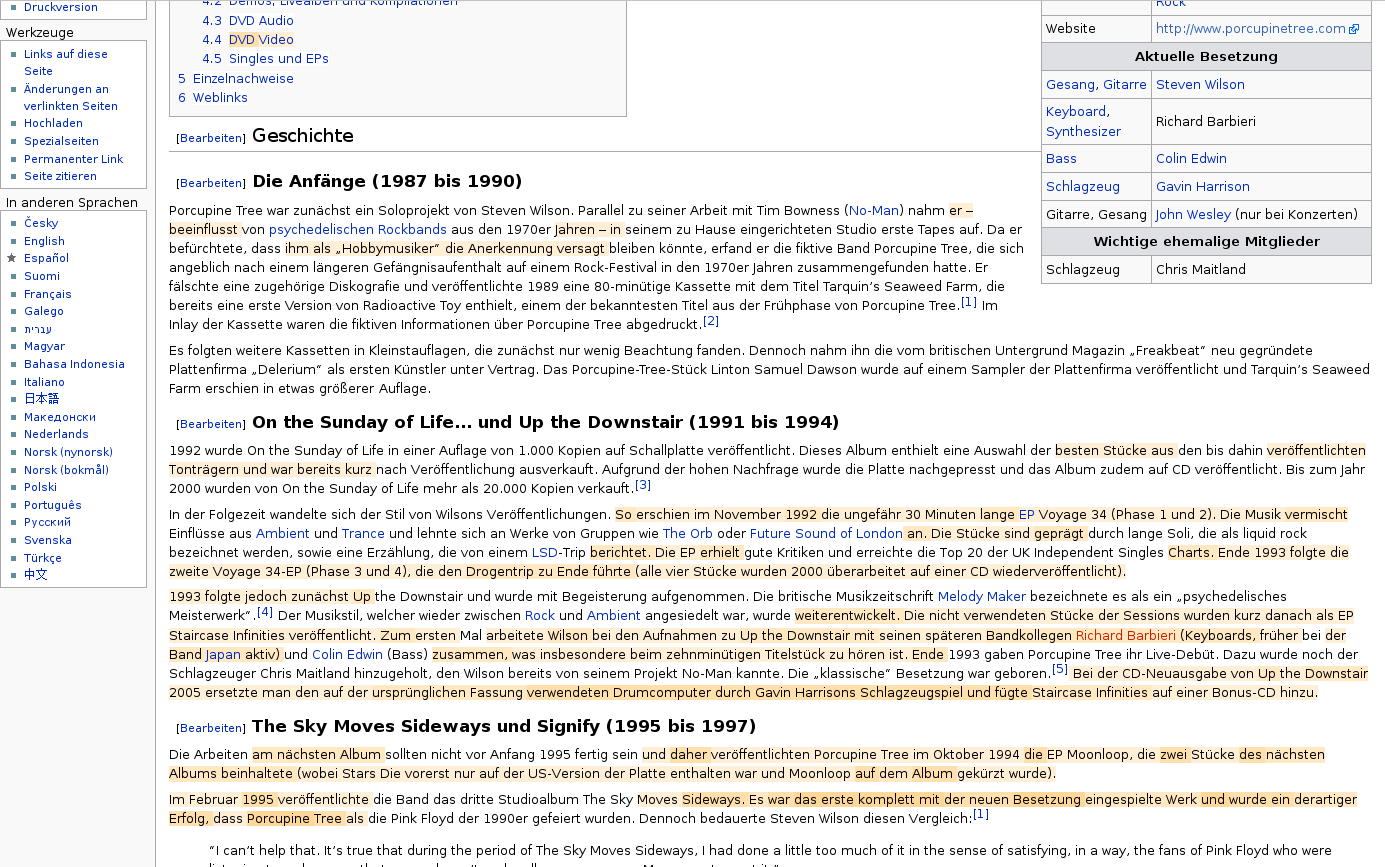
\includegraphics[width=0.8\textwidth,clip=true,resolution=300]{img/wikitrust.jpg}
         \caption{Wikitrust in action (2011)}
         \label{fig:wikitrust}
       \end{figure}

 \cite{Lucassen2011} 

        \section{Conclusions}
        Possible extensions.  Perhaps we can examine more about what
        we may find out about the articles. Cite other studies Lih's
        2004 study of articles immediately after they have been cited
        in the press\cite{Lih2004}, and Metyan's 2012 use of the site
        to predict box-office success \cite{Mestyan2012}. Lieberman
        worked out their locale.\cite{Lieberman2009}:

        \begin{enumerate}
          \item peaks in activity (rate of levenshtein distance... may
            have to be in a log graph...)
          \item 
        \end{enumerate}

        PREDIFINED / NOT-PREDEFINED ideas of quality. look for when
        the the article levels off? And do this by DATE rather than
        REVISION. We may assume that pageviews are more
        well-distributed than revisions

        summarize major contributions (which do we care about?)
        evaluate your current position point out any flaw in
        methodology/research/contradictions are there any gaps in the
        area which you will cover in your research?  How will you
        integrate sources you have mentioned into your dissertation?
        Point out any areas for further study

        \begin{figure}[h!]
          \centering
          \begin{tikzpicture}
            \matrix (m) [matrix of math nodes, row sep=4em, column
              sep=4em] { & v_i & \\ v_{i-1} & & v_{i+1}\\ };
            \path[-stealth] (m-2-1) edge node [left]
                 {$ed(v_{i-1},v_i)$} (m-1-2) edge node [below]
                 {$ed(v_{i-1},v_{i+1})$} (m-2-3) (m-1-2) edge node
                 [right] {$ed(v_i,v_{i+1})$} (m-2-3); 
                 \draw[color=red]
                 (m-1-2.north west) -- (m-1-2.north east) --
                 (m-1-2.south east) -- (m-1-2.south west) --
                 (m-1-2.north west);
          \end{tikzpicture}
          \\$ed(v_{i-1},v_i) < ed(v_{i-1},v_i) + ed(v_{i},v_{i+1})$
          \caption{Diagram showing identification of a partially
            undone operation}
          \label{fig:part-undo}
        \end{figure}

        \begin{figure}[h!]
          \centering
          \begin{tikzpicture}
            \matrix (m) [matrix of math nodes, row sep=4em, column
              sep=4em] { & v_i & \\ v_{i-1} & & v_{i+1}\\ };
            \path[-stealth] (m-2-1) edge node [left]
                 {$ed(v_{i-1},v_i)$} (m-1-2) edge node [below]
                 {$ed(v_{i-1},v_{i+1})$} (m-2-3) (m-1-2) edge node
                 [right] {$ed(v_i,v_{i+1})$} (m-2-3); 
                 \draw[color=red]
                 (m-1-2.north west) -- (m-1-2.north east) --
                 (m-1-2.south east) -- (m-1-2.south west) --
                 (m-1-2.north west);
          \end{tikzpicture}
          \\$ed(v_{i-1},v_{i+1}) = 0$, $ed(v_{i-1},v_{i}) > 0$)
          \caption{Diagram showing identification of an undone operation}
          \label{fig:undo}
        \end{figure}

        We will also consider introducing ways of representing the
        history of a page in space. The position of a certain revision
        in that space may help us define the corresponding edit operation.

        Since we are taking one revision, say, the current one, to be
        the ultimate 'target' of previous edits, perhaps we should
        describe all previous edits in terms of this final version. We
        may measure the edit distance between all previous versions
        and arrive at the set:
        
        \begin{figure}[h!]
          \centering
          $\text{prev} = <ed(v_0,v_n),ed(v_1,v_n),...,ed(v_n,v_n)>$  
        \end{figure}
        where $v_n$ is the 'target' version of a page, and we are
        considering $n$ revisions of the page

        %% \begin{figure}[h!]
        %%   \centering
        %%   \begin{tikzpicture}
        %%     \matrix (m) [matrix of math nodes, row sep=4em, column
        %%       sep=4em] { & v_i & \\ v_{i-1} & & v_{i+1}\\ };
        %%   \end{tikzpicture}
        %%   \\$ed(v_{i-1},v_{i+1}) = 0$, $ed(v_{i-1},v_{i}) > 0$)
        %%   \caption{Diagram showing revisions}
        %%   \label{fig:}
        %% \end{figure}
        

        \section{Progress report}
        
        The Code in appendix A


\clearpage
\printbibheading[heading=bibintoc,title={References}]
\printbibliography[keyword=wiki,heading=subbibliography,title={Wikipedia}]
\printbibliography[keyword=edit,heading=subbibliography,title={Edit
distance}]

        
\clearpage
\begin{appendices}
\section{Appendix A: Code progress}
\subsection{Python class for scraping a Wikipedia article's revision history}
The following code is a first draft of a class which incrementally
traces, parses, and stores the revision history of select articles. It
chooses random articles up to a maximum amount of articles unless an
article (or articles) are specified. It traces the entire
discoverable\footnote{Using the Wikipedia API, articles can either be
  traced back to their origin (revision parent ID = 0), or to the
  point at which a loop is found in the revision history - this
  usually happens with older articles.} history of the, unless a
specific depth is specified by the user.

The class already yields workable data, but here is some immediate
further work for this code:
\begin{itemize}
  \item Allow the user to specify timeframe
  \item Allow for integration with a postgres database (at the moment
    the code saves the data in CSV format).
\end{itemize}

This code is an extension to an existing wikipedia API class for
python (which did not provide the features we need
here).\cite{python-wikipedia}

\lstinputlisting[language=Python,frame=single]{../wikiScraper/WikiRevisionScrape.py}
\subsection{Example output}
\fvset{frame=single}
\VerbatimInput{../wikiScraper/output.txt}

\clearpage
\section{Appendix B: Python class for basic, space-naive Levenshtein
  implementation}
\subsection{Code}
\lstinputlisting[language=Python,frame=single]{../lshtein/basic/LevDistBasic.py}
\subsection{Example output}
\fvset{frame=single}
\VerbatimInput{../lshtein/basic/output.txt}
\end{appendices}

\end{document}
